\subsection{Sơ đồ tuần tự}
% https://www.uml-diagrams.org/sequence-diagrams.html
\FloatBarrier
\begin{figure}[h]
	\begin{center}	
		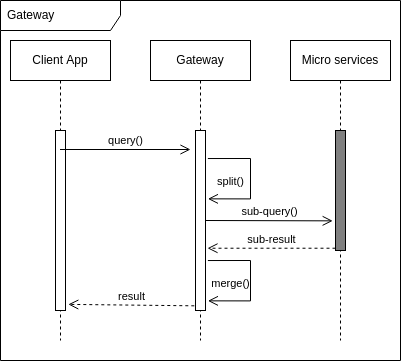
\includegraphics[width=0.8\textwidth]{sequence-gateway}
		\caption{Sơ đồ tuần tự hoạt động của gateway}
	\end{center}

Giải thích:
\begin{enumerate}
	\item Một truy vấn đồ thị từ ứng dụng khách sẽ gửi đến gateway.
	\item Gateway sẽ phân tích ra thành các đồ thị con cho các máy chủ dịch vụ tương ứng
	\item Các máy chủ dịch vụ nhận và thực hiện các tuy vấn với cơ sở dữ liệu.
	\item Khi nhận được dữ liệu từ các máy chủ dịch vụ, gateway sẽ gộp lại và gửi cho ứng dụng khách.
\end{enumerate}
\end{figure}

\clearpage
\FloatBarrier
\begin{figure}[!htbp]
	\begin{center}	
		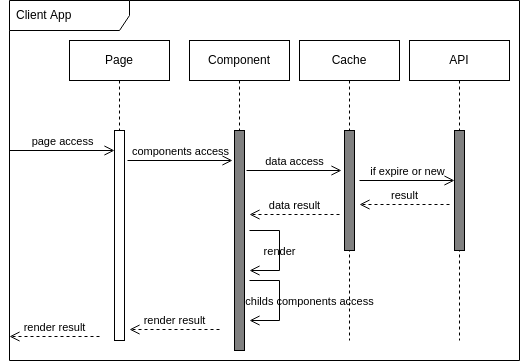
\includegraphics[width=\textwidth]{sequence-component}
		\caption{Sơ đồ tuần tự kết xuất giao diện}
	\end{center}
Giải thích:
\begin{enumerate}
	\item Người dùng truy cập vào trang của ứng dụng khách.
	\item Trang sẽ truy cập đến components của cấu trúc react.js
	\item Khi component được kết xuất thành công sẽ gọi lấy dữ liệu từ bộ nhớ cache
	\item Bộ nhớ cache thông qua truy vấn từ component sẽ sử dụng làm cache-key để lấy dữ liệu cũ hoặc gọi dữ liệu mới từ máy chủ.
	\item Kết quả trả về lại cho component tái kết xuất.
	\item Khi kết xuất nếu có gọi đến component con thì tiếp tục quá trình 2
	\item Sau quá trình kết xuất hoàn tất thì trả dữ liệu cho màn hình hiển thị.
\end{enumerate}
\end{figure}

\clearpage
\FloatBarrier
\begin{figure}[!htbp]
 	\centering
	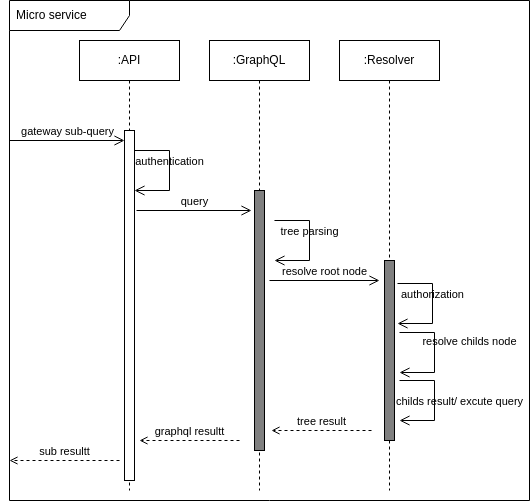
\includegraphics[width=0.8\textwidth]{sequence-service}
	\caption{Sơ đồ tuần tự xử lí truy vấn}
	Giải thích:
	\begin{enumerate}
		\item Một truy vấn từ Gateway đến máy chủ dịch vụ sẽ được định danh tại lớp API.
		\item Sau đó nội dung truy vấn sẽ được gửi đến lớp GraphQL.
		\item Lớp GraphQL đóng gói truy vấn thành một cây dữ liệu và gửi cho lớp Resolver giải quyết.
		\item Lớp Resolver quét qua tất cả các nút và quy nạp kết quả.
		\item Dữ liệu được trả về cho GraphQL và tiếp tục trả cho lớp API để phản hồi cho máy chủ gateway.
	\end{enumerate}
\end{figure}

